\documentclass[fancy,phd,twoside]{byuthesis}
% Class options are simple/fancy and masters/phd.
% Leave options blank for defaults.
% Defaults are simple for document style, and masters for degree type.


%%%%%%%%%%%%%%%%%%%%%%%%%%%%%%%
% Custom options and packages %
%%%%%%%%%%%%%%%%%%%%%%%%%%%%%%%
% Define path to figure files
\graphicspath{{figures/}}

% Define sequences of Latin text to fill space in example documents
% (not needed for your thesis -- delete or comment out if you'd like)
\usepackage{blindtext} 


%%%%%%%%%%%%%%%%%%%%%%%%%%%%%%
% Define title page elements %
%%%%%%%%%%%%%%%%%%%%%%%%%%%%%%
% Thesis title for required BYU title page
% On the required BYU title page, multiple-line titles should MUST be formatted into an inverted
% pyramid style. Choose line breaks accordingly.
\title{Exceptional Engineering Research That Has Taken Longer \\ Than Everyone Thought It Would}

% On the custom title page, use the same title, but format as you like
\customtitle{Exceptional Engineering Research \\ That Has Taken Longer Than \\ Everyone Thought It Would}

% Your name goes here:
\author{Emma J. Student}

% This is the date of graduation
\date{April 2021}

% If your degree is not a PhD or MS, then you can overwrite the degree using 
% the \degree command: \degree{Bachelors of Basics}

% Your department
\department{Department of Electrical and Computer Engineering}

% The names of your committee members
\committeechair{Norman D. Smith}
\committeemember{Mary Q. Scott}
\committeemember{Steven R. Jones}
\committeemember{Anna B. Hanna}

% Include any keywords you would like for your thesis/dissertation
\keywords{awesome stuff, killer app, buzz words}


%%%%%%%%%%%%%%%%%%%%%%%%%%%%%%%%%%
% ---Bibliography source file--- %
%%%%%%%%%%%%%%%%%%%%%%%%%%%%%%%%%%
%  Default is references.bib 
\bibliography{references}


%%%%%%%%%%%%%%%%%%%%%%%%%%
% --- Begin Document --- %
%%%%%%%%%%%%%%%%%%%%%%%%%%
\begin{document}


%%%%%%%%%%%%%%%%%%%%%%%%%%%%%%%%%%%%%%%%%%%%%%%%%%%%%%%
% --- Front matter (probably don't need to change)--- %
%%%%%%%%%%%%%%%%%%%%%%%%%%%%%%%%%%%%%%%%%%%%%%%%%%%%%%%
	\frontmatter
	
	\titlepage
	\cleartooddpage

	\customtitlepage
	\cleartooddpage

	\begin{abstract}  
	The abstract is summary of the work with emphasis on the findings of the study. It is not intended to be an {\em introduction} to the research.
	Instead, it should concisely state the problem addressed, the methods developed and used, and the results obtained. It must be single spaced and no
	more than one page in length. It must use the same font and font size as the rest of the work. The abstract precedes the acknowledgment page and
	the body of the work.
	{\color{mediumgray} \blindtext}
\end{abstract}
	\cleartooddpage

	\begin{acknowledgments}
	Students should acknowledge funding sources. They may also use the acknowledgment page to express appreciation for the committee members, friends or family who provided support or aided the research, writing or technical aspects of the thesis/dissertation. Acknowledgments should be simple and in good taste.
	{\color{mediumgray} \blindtext}
\end{acknowledgments}

	\cleartooddpage

	\pdfbookmark{Table of Contents}{tableofcontents}
	\tableofcontents*
	\cleartooddpage

	\listoffigures
	\cleartooddpage

	\listoftables
	\cleartooddpage

	\nomenclature{$c$}{Speed of light in a vacuum inertial frame}
\nomenclature{$h$}{Planck constant}
\nomenclature{$\mathit{Re}$}{Reynolds number}
\nomenclature{$\mathbf{x}$}{State vector}
\nomenclature{$\alpha$}{Angle of attack}
\nomenclature{$\beta$}{Sideslip angle}
\nomenclature{$\gamma$}{Climb angle}
\nomenclature{$p$}{Roll rate}
\nomenclature{$q$}{Pitch rate}
\nomenclature{$r$}{Yaw rate}

\printnomenclature
	\clearpage


%%%%%%%%%%%%%%%%%%%%%
% --- Main Body --- %
%%%%%%%%%%%%%%%%%%%%%
	\mainmatter
	
% Here you want to include the .tex files where you have your chapter content.  
% You can name the files whatever you want, but make sure that what you call 
% them here matches what you name them.
%
% Note that the chapter .tex files for the simple template and fancy template 
% are different because fancy template option has commands and features not 
% available in the simple template option. 

% Fancy Version
	\chapter{Introduction}
\label{ch:intro}

The opening chapter of a thesis or dissertation will typically provide an introduction to the body of research. At the beginning of a chapter, it is common to provide some introductory text. Instead of discussing research, this template document will highlight how the {\ttfamily byuthesis.cls} and \LaTeX{} can be used to prepare a thesis or dissertation document for submission in the College of Engineering at BYU. A concise statement of the College of Engineering formatting requirements can be found in Appendix~\ref{app:format}.

\section{Class Options}
\label{sec:class_options}
The {\ttfamily byuthesis} class has two class options. The first option allows the author to choose between a {\em simple} or {\em fancy} document format. The simple format is traditional and straightforward and can be implemented in standard word processor. The fancy format leverages the advanced typesetting features of \LaTeX{} and the {\ttfamily memoir} class that more effectively utilizes the full letter-size page while following typesetting best practices. With the second option, the author can specify whether the document fulfills the requirements for a masters or doctoral degree. For example, to use the {\ttfamily byuthesis} class for a doctoral dissertation in the simple format, the class definition would be \verb|\documentclass[simple,phd]{byuthesis}|. To create a masters thesis in the the fancy format, the definition would be \verb|\documentclass[fancy,masters]{byuthesis}|. The example template document ({\ttfamily template.tex}) can be compiled using any combination of these options. Note that the simple and fancy formats use different source files for the chapters in this document. Be sure to uncomment the appropriate {\ttfamily chap*.tex} files in {\ttfamily template.tex}.

\section{Styles}
\label{sec:intro_styles}
The formatting and \LaTeX{} features that you will use to prepare your thesis are outlined briefly in the next several chapters. The narrow, single column format of this document is based on long-standing principles of typography~\autocite{Bringhurst19}. This formatting is easy to read compared to the wide-column, double-spaced format used previously. The format of the document is defined in {\ttfamily byuthesis.cls}, a \LaTeX{} class defined specifically for theses and dissertations in the College of Engineering at BYU. To give a better sense of the format of the document, we will occasionally throw in some random Latin text to take up white space. We set it apart from the text requiring your attention with a grey font color.

\myshorttext

When using the {\ttfamily byuthesisfancy.cls}, footnotes appear as sidenotes in the right margin.\sidenote{This is a sidenote created with the {\ttfamily $\backslash$sidenote} command.} You can make a reference to a section by using its label, such as~\cref{sec:intro_styles}. You can reference a chapter in this way, for example~\cref{ch:intro}. Here is an example of a citation of a master's thesis~\autocite{masters1}. References for this template document are held in a file called {\ttfamily references.bib}.

\subsection{Including Figures and Tables}
The syntax above provides an example for declaring a subsection. This subsection will include some text and give an example of a figure and a table. Let's start with with a figure. Figure~\ref{fig:gradf_half_space} shows the gradient of a function and the halfspace where the function is decreasing. Notice how the \verb|\ref| command automatically references the correct figure number. Notice also that the \verb|~| inserts a non-breaking space, so that the label Figure and the figure number are never separated by a line break.

\begin{figure}[htbp]
	\centering
	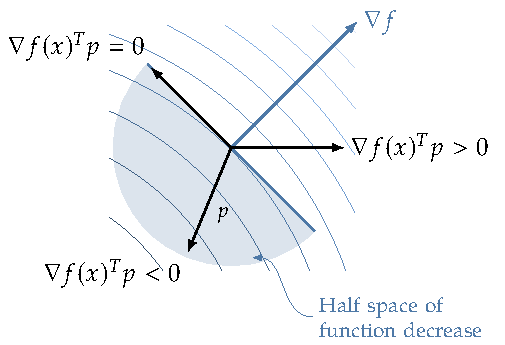
\includegraphics[width=3.0in]{gradf_half_space}
	\caption{This is a regular figure with a centered bottom caption.}
	\label{fig:gradf_half_space}
\end{figure}

\myshorttext

With the {\ttfamily byuthesis.cls} document class, we can have small figures that are set in the sidemargin. Figure~\ref{fig:brach} is an example of a margin figure.
\begin{marginfigure}
	\includegraphics[width=1.8in]{brachistochrone}
	\caption{This is an example of a margin figure.}
	\label{fig:brach}
\end{marginfigure}

\myshorttext

We can also create figures that place the caption in the side margin. This is a matter of personal preference.
\begin{figure}[htbp]
	\begin{sidecaption}{This is a figure with a side caption that is not short, but not that long either.}[fig:sidecap]
		\centering
		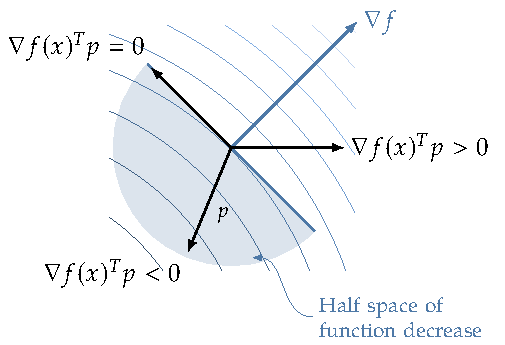
\includegraphics[width=3.5in]{gradf_half_space}
	\end{sidecaption}
\end{figure}

Finally, we can create a figure that spans the width of the text column and the side margin. This option should not be used frequently as it requires some tweaking of the vertical distance of the caption and follow-on text below the figure. It will work robustly when the figure appears at the top or middle of a page, but may push the caption onto the next page when it appears at the bottom. There may be some instances with wide images where the additional manual adjusting is worth the effort.

\begin{figure}[h]
	\setlength{\sidecapraise}{-1.3cm}   % manual adjustment of figure caption position
	\begin{sidecaption}{The caption for a full-width figure appears in the margin below it.}[fig:fullwidth] %Such figures utilize the side margin.}
		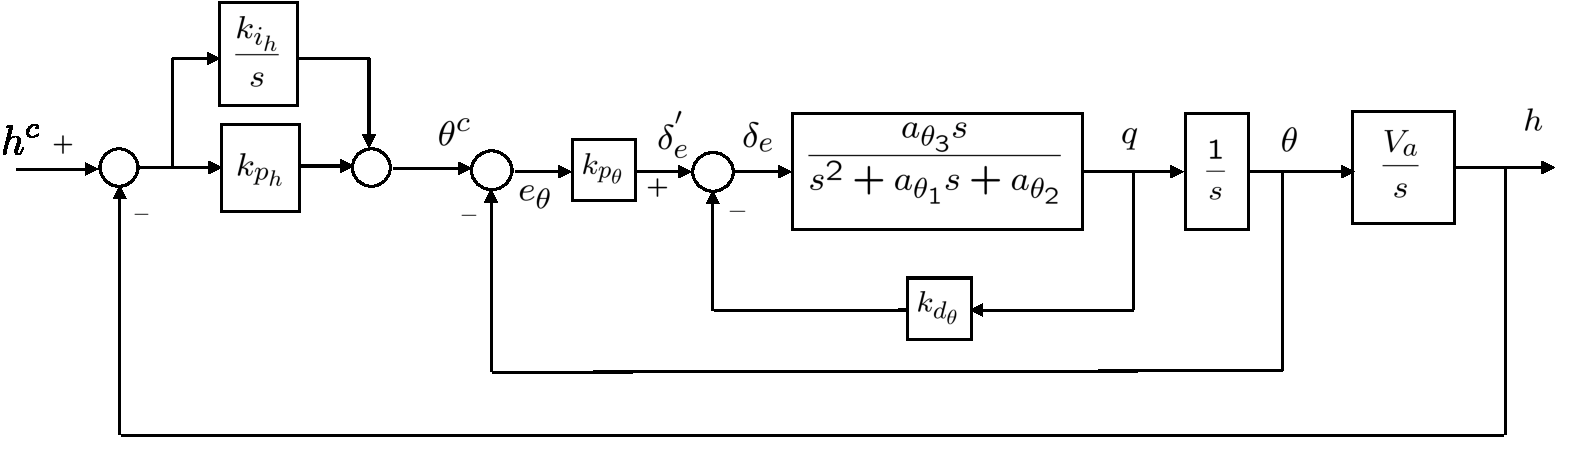
\includegraphics[width=1.35\textwidth]{altitude-pitch-all}
	\end{sidecaption}
	\vskip -1.7cm     % manual adjustment of position of main text below figure   
\end{figure}

\subsubsection{Subsubsection Example}
The syntax above provides an example of how to include a subsubsection. In this thesis template, the document has four primary division levels: \verb|\chapter|, \verb|\section|, \verb|\subsection|, and \verb|\subsubsection|. The command \verb|\subsubsection| is used to define the lowest level of division. Notice that subsubsection titles are not numbered.

\subsubsection{Including Tables}
Tables are also fairly straightforward to include in a \LaTeX{} document. Table~\ref{tab:table_example} shows a simple table. \LaTeX{} refers to figures and tables as floats and often tries to locate figures at the top or bottom of a page. The user has some control over this, but \LaTeX{} can behave like it has a mind of its own sometimes. In reality it is placing figures according to internal algorithms and parameters that you can adjust. If you are interested in digging into this level of detail, an internet search on ``LaTeX float parameters'' will provide ample reading.  In creating the table, we have used the command \verb|\begin{table}[t]|. The parameter \verb|[t]| allow us to specify preference for the location of table to be at the \emph{top} of the page.

\begin{table}[t]
	\centering
	\caption{This is a standard table with a top caption.}
	\label{tab:table_example}	\begin{tabular}{ c c c c}
		\toprule
		basin & curve \\
		name & number & minimum & maximum \\
		\midrule
		1B & 68.5 & 49.2 & 84.1 \\ 
		2B & 66.2 & 46.8 & 82.7 \\ 
		3B & 65.4 & 45.5 & 82.3 \\
		\midrule
		average & 66.7 & 47.2 & 83.0 \\
		\bottomrule
	\end{tabular}
\end{table}

Table~\ref{tab:table_sidecaption} shows an example of the same table using a side caption. We have used the placement preferences \verb|[thb]| to give first preference to the top of the page, second preference to the current positioning in the source code (\emph{here}), and third preference to the \emph{bottom} of the page. As you can see, \LaTeX{} may override our preferences, based on the space available and its typesetting rules.
\begin{table}[thb]
	\begin{sidecaption}{This is a standard table with a side caption.}[tab:table_sidecaption]
		\centering
		\begin{tabular}{ c c c c}
			\toprule
			basin & curve \\
			name & number & minimum & maximum \\
			\midrule
			1B & 68.5 & 49.2 & 84.1 \\ 
			2B & 66.2 & 46.8 & 82.7 \\ 
			3B & 65.4 & 45.5 & 82.3 \\
			\midrule
			average & 66.7 & 47.2 & 83.0 \\
			\bottomrule
		\end{tabular}
	\end{sidecaption}
\end{table}

\subsection{Formatting Equations}
Equation formatting is one of \LaTeX's most useful features and a good reason why it is often used for theses and dissertations in the College of Engineering. It is easy to format equations within a sentence, such $c = 2 \pi r$ to describe the circumference of a circle. Equations should be treated as part of the text. As an example, the surface area of a cylinder is given by 
\begin{equation}
	\label{eq:surface_area_cyl}
	S = 2\pi r \left( r + h \right) , 
\end{equation}
where $r$ is the radius of the cylinder and $h$ is its height. The area of a circle can be expressed in terms of its diameter $d$ as 
\begin{equation}
	\label{eq:area_circle}
	A = \frac{\pi}{4} d^2 .
\end{equation}

Often, it is desirable to align a sequence of equations. Again, \LaTeX{} makes this pretty easy. The roots of the polynomial function $f(x)$ can be found by factoring
\begin{align}
	f(x) &= x^3 + 5x^2 + 6x \\
		 & = x (x^2 + 5x + 6) \\
		 & = x (x + 2)(x +3) ,
\end{align}
setting each of the factors to zero, and solving for $x$. Equations without numbers can be typeset like this
\[
	x = a + b
\]
or like this
\begin{equation*}
	y = c + d .
\end{equation*}
Just as we did with sections, figures, and tables, we can reference a specific equation by using its declared label. In~\eqref{eq:surface_area_cyl}, the surface area of a cylinder is defined. Another format would be to say Equation~\ref{eq:area_circle} defines the area of a circle. Yet another format is \cref{eq:area_circle}. Any of these formats is acceptable. Use just one of them and be consistent.

\LaTeX{} can do so much with the typesetting of equations. These few examples are just a small sampling of its impressive capabilities.


	\chapter{Additional \rmfamily{\LaTeX{}} Formatting}
\label{ch:ch2}

In this chapter, we'll provide some additional guidelines and useful \LaTeX{} commands for formatting your document.


%{\color{mediumgray} \blindtext}
\section{More {\rmfamily\LaTeX{}} Usage Examples}
In Figure~\ref{fig:brach2} below, we show some pretty blue and grey lines. This is the first figure in \cref{ch:ch2} and you can see that it is numbered accordingly. Notice that the \verb|\ref| command automatically provides the correct numbering for the item being referenced. If you use the \verb|\cref| command, the label (e.g., Figure, Chapter) will be added automatically. For figures and equations, however, \verb|\cref| will abbreviate the labels (i.e., Fig. and Eq.). Either \verb|\ref|, with label provided by you, or \verb|\cref|, with automatic labeling, can be used. 

\begin{figure}[htbp]
	\centering
	\includegraphics[width=2.2in]{figures/brachistochrone}
	\caption[Short caption to appear in list of figures.]{This is another figure. Some authors have paragraph-like descriptions of their figures that they put into the caption. This is acceptable, but readers don't really want or need a super long caption showing up in their list of figures. The {\ttfamily caption} command provides a nice solution.}
	\label{fig:brach2}
\end{figure}

\section{Bibliography}
Another great feature of \LaTeX{} is that it allows you to create a list or database of books, papers, and other documents that you can easily cite in your document. In engineering, it is common to give your bibliography list the title References and we will follow that convention. \LaTeX{} automatically numbers the citations and builds a bibliography for you.\sidenote{The building of your bibliography is actually done by the {\ttfamily biblatex} package. If you use an IDE to work with \LaTeX, this may not be obvious to you.} The bibliography is typeset according the style you specify. We recommend the {\em IEEEtran} bibliography style that produces a numbered list in order of citation. For this document, the file {\ttfamily references.bib} contains the bibliographic reference information that's available for citation in the thesis document. Each reference is given a cite key (a label) that is used to cite the reference. For example, here is a reference to a book~\autocite{book1} and a reference to a doctoral dissertation~\autocite{doctoral1}. Journal articles~\autocite{journal1}, are treated differently than conference papers~\autocite{conference1} since their references require slightly different information. For each reference entry in your {\ttfamily .bib} file, different information fields will have to be populated. Examples of these fields include, {\em author}, {\em title}, {\em year}, and so on. Different types of publications will have different required fields for you to fill out. There are other types of citations that you may use, such as book chapters and websites. You can manually edit your {\ttfamily .bib} file with a text editor, or you can use one of the several popular apps that are available for editing and organizing your bibliography information.

\section{Use of Units}
Units should be appropriately used for all measurements and data presented in the document. Standard abbreviations for units (e.g., m for meters, N for newtons, in. for inches) should be used whenever data is presented. For example, the shaft was 1.23 cm in diameter. Notice that there is a space between the number and the unit, and the unit is typeset in vertical (roman) text and is {\em not italicized}. Italics is reserved for emphasis and for mathematical variables. Periods are not used after abbreviations except in the special case of the abbreviation for inches as in. to avoid confusion with the word in. Units are typically spelled out when they are used without data. For example, newtons are a measure of force, while kilograms are a measure of mass.

\section{Capitalization of Reference Labels}
Throughout your document, you will refer to figures, tables, equations, chapters, appendices, and sections by name (e.g., Figure 2.1, Section 3.4, Equation 2.1, and so on). You may choose to capitalize these reference labels, or to leave them uncapitalized (e.g., figure 2.1, section 3.4, equation 2.1). The choice is yours, just be consistent -- all reference labels should be capitalized, or uncapitalized.

\section{Algorithms}
Software and algorithm development can play an important role in graduate research. Rather than including software code, particularly in the body of the thesis, presenting your algorithms in the form of pseudo-code may be more desirable. The {\ttfamily algorithm} package in \LaTeX{} provides tools for clearly presenting your algorithms. A simple example of the use of this package is presented in Algorithm~\ref{alg:ekf}.

\begin{algorithm}
	\caption{{\color{black} Continuous-discrete extended Kalman filter.}} \label{alg:ekf}
	\begin{algorithmic}[1]
	    \State Initialize:  $\hat{x} = 0$.
	    \State Pick an output sample rate $T_{\textit{out}}$ that is much less than
	    the sample rates of the sensors.
	    \State At each sample time $T_{\textit{out}}$:
	    \For{$i=1$ to $N$}
	        \State $\hat{x} = \hat{x} + \left(\frac{T_{\textit{out}}}{N}\right) \left( f(\hat{x}, u)\right)$
	        \State $A = \frac{\partial{f}}{\partial{x}}$
	        \State $P = P + \left(\frac{T_{\textit{out}}}{N}\right)
	        \left(AP+PA^T + GQG^T\right)$
	    \EndFor
	    \If{a measurement has been received from sensor $i$}
	        \State $C_i = \frac{\partial{c_i}}{\partial{x}}$
	        \State $L_i = PC_i^T(R_i+C_iPC_i^T)^{-1}$
	        \State $P = (I-L_iC_i)P$
	        \State $\hat{x} = \hat{x} +  L_i\left( y_i - c_i( \hat{x})
	        \right)$.
	    \EndIf
	\end{algorithmic}
\end{algorithm}

\section{Landscape Drawings and Tables}
If you have a figure or table that is best presented in landscape format on a full page, the {\ttfamily rotating} package in \LaTeX{} provides a convenient way to do this. Figure~\ref{fig:landscape_dwg} on the following page shows an example a landscape-format drawing.
\begin{sidewaysfigure}
	\centering
	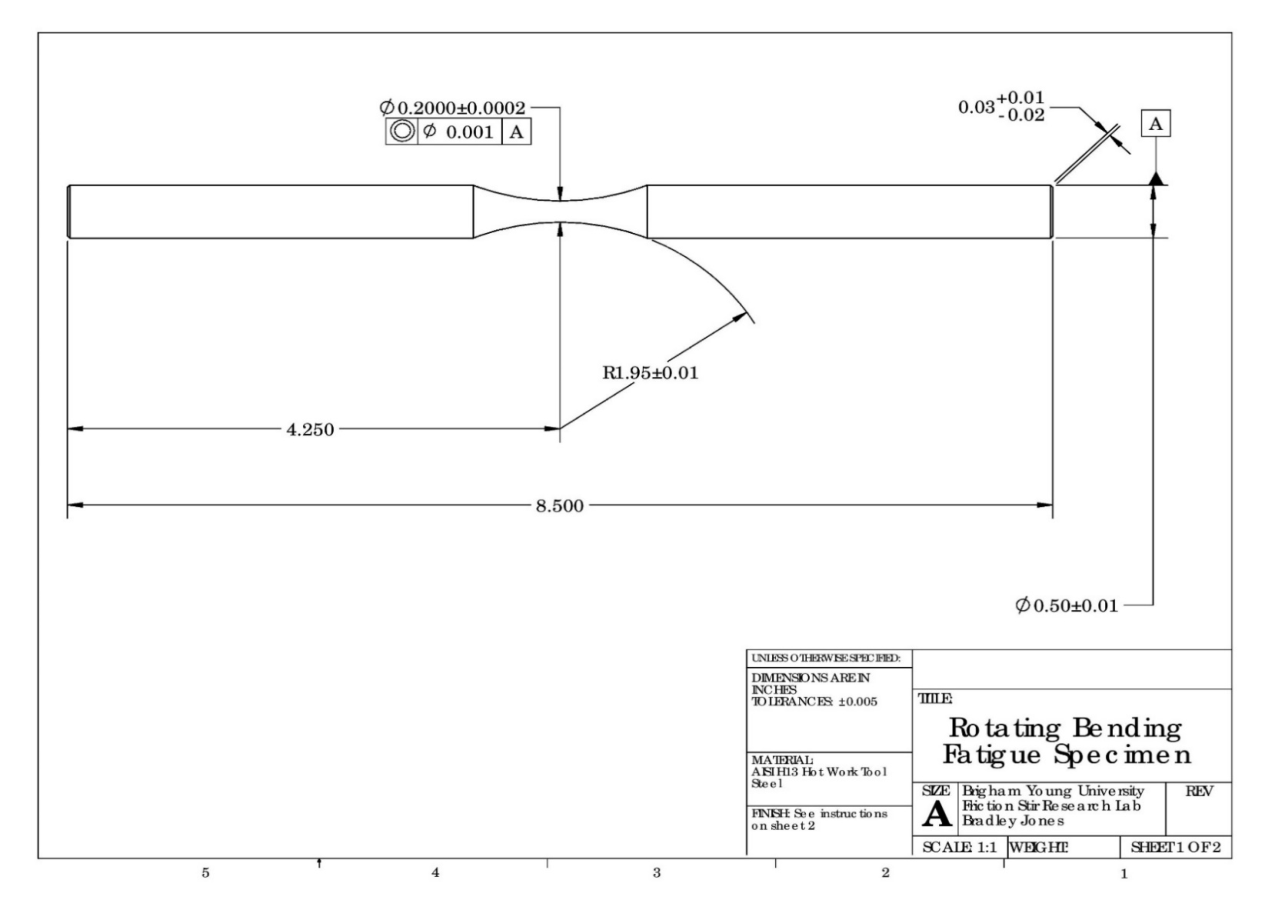
\includegraphics[width=0.7\textwidth]{figures/part_dwg_landscape.pdf}
	\caption{Example of full-page landscape drawing.}
	\label{fig:landscape_dwg}	
\end{sidewaysfigure}



	\chapter{Article-based Chapters}
\label{ch:article_based_chap}

With the allowed changes in thesis and dissertation formatting, BYU Graduate Studies
now allows students to insert journal or conference articles as chapters into their
thesis/dissertation document. To do so, the student must be a primary author. The
formatting of an article-based chapter must be fully consistent with the formatting
defined in this document with chapter, section, equation, figure, and table numbering
integrated accordingly. Article-based chapters must include a complete citation and
the following statement: ``I hereby confirm that the use of this article is compliant
with all publishing agreements.'' The paragraph below is an example of how this could
be done. It should appear immediately following the chapter title.

\noindent This chapter is composed from a paper entitled ``Really great research from
a BYU engineering student'' published in the journal Awesome Engineering~\cite{StudentRP20}.
I hereby confirm that the use of this article is compliant with all publishing agreements.

\section{Some Additional Comments}
The publication of a conference or journal article is a significant milestone for a graduate 
student and should be an objective for all students pursuing graduate research in the College 
of Engineering. We encourage the use of article-based chapters in theses and dissertations 
provided that it aligns with the goals and objectives of the research. Articles, however, 
are often constrained in length forcing the exposition to be more concise or narrow in 
scope than may be desired for the intended audience of the thesis/dissertation. For example, 
if an objective is to guide the learning of subsequent graduate-student researchers, it 
may be beneficial to include additional details or a broader discussion that may be more 
tutorial in nature. Often more results from a wider variety of cases would be included 
in a dissertation or thesis than would be possible in a journal or conference publication. 
Your graduate committee will help guide your efforts in these matters.

	\chapter{Conclusions}

The purpose of this template is to provide basic instructions in creating your dissertation/thesis document. If you need assistance with writing, please visit the Writing Center in the JKB or consult with your advisor. If you need assistance with \LaTeX, there are tutorials and ample documentation online. You may want to consult with your graduate-student peers who use \LaTeX. If you discover something that would make this template more useful, please feel free to make recommendations.

Regardless of whether this template or some other method of formatting is employed, you (the student) are responsible for following the guidelines found in \cref{ap:format}. Below is a brief checklist of things to look for as you review your thesis for formatting:
\begin{itemize}
	\item Check numbering of sections, figures, tables, equations to make sure they are consistent.	This is where you will be really glad that you are using \LaTeX.
	\item Ensure that your table of contents, list of figures, and list of tables are up to date and that page numbers are correct. (Hurray for \LaTeX!)
	\item Make sure all pages are numbered, beginning with the table of contents.
	\item Be sure there is no more than 1 inch of extra white space at the bottom of any page (in addition to the 1-inch margin) except for the final page of a chapter.
	\item Make sure there are no widows or orphans.\footnote{A \emph{widow} occurs when the last line of a paragraph ends up on the first line of a page. An \emph{orphan} occurs when the first line of a paragraph appears on the last line of a page. Your document may require manual tweaking when it is in final form to get rid of widows and orphans.}
\end{itemize}



% Simple Version
%	\chapter{Introduction}
\label{ch:intro}

The opening chapter of a thesis or dissertation will typically provide an introduction to the body of research. At the beginning of a chapter, it is common to provide some introductory text. Instead of discussing research, this template document will highlight how the {\ttfamily byuthesis.cls} and \LaTeX{} can be used to prepare a thesis or dissertation document for submission in the College of Engineering at BYU. A concise statement of the College of Engineering formatting requirements can be found in Appendix~\ref{app:format}.

\section{Class Options}
\label{sec:class_options}
The {\ttfamily byuthesis} class has two class options. The first option allows the author to choose between a {\em simple} or {\em fancy} document format. The simple format is traditional and straightforward and can be implemented in standard word processor. The fancy format leverages the advanced typesetting features of \LaTeX{} and the {\ttfamily memoir} class that more effectively utilizes the full letter-size page while following typesetting best practices. With the second option, the author can specify whether the document fulfills the requirements for a masters or doctoral degree. For example, to use the {\ttfamily byuthesis} class for a doctoral dissertation in the simple format, the class definition would be \verb|\documentclass[simple,phd]{byuthesis}|. To create a masters thesis in the the fancy format, the definition would be \verb|\documentclass[fancy,masters]{byuthesis}|. The example template document ({\ttfamily template.tex}) can be compiled using any combination of these options. Note that the simple and fancy formats use different source files for the chapters in this document. Be sure to uncomment the appropriate {\ttfamily chap*.tex} files in {\ttfamily template.tex}.

\section{Styles}
\label{sec:intro_styles}
The formatting and \LaTeX{} features that you will use to prepare your thesis are outlined briefly in the next several chapters. The narrow, single column format of this document is based on long-standing principles of typography~\autocite{Bringhurst19}. This formatting is easy to read compared to the wide-column, double-spaced format used previously. The format of the document is defined in {\ttfamily byuthesis.cls}, a \LaTeX{} class defined specifically for theses and dissertations in the College of Engineering at BYU. To give a better sense of the format of the document, we will occasionally throw in some random Latin text to take up white space. We set it apart from the text requiring your attention with a grey font color.

\myshorttext

When using the {\ttfamily byuthesisfancy.cls}, footnotes appear as sidenotes in the right margin.\sidenote{This is a sidenote created with the {\ttfamily $\backslash$sidenote} command.} You can make a reference to a section by using its label, such as~\cref{sec:intro_styles}. You can reference a chapter in this way, for example~\cref{ch:intro}. Here is an example of a citation of a master's thesis~\autocite{masters1}. References for this template document are held in a file called {\ttfamily references.bib}.

\subsection{Including Figures and Tables}
The syntax above provides an example for declaring a subsection. This subsection will include some text and give an example of a figure and a table. Let's start with with a figure. Figure~\ref{fig:gradf_half_space} shows the gradient of a function and the halfspace where the function is decreasing. Notice how the \verb|\ref| command automatically references the correct figure number. Notice also that the \verb|~| inserts a non-breaking space, so that the label Figure and the figure number are never separated by a line break.

\begin{figure}[htbp]
	\centering
	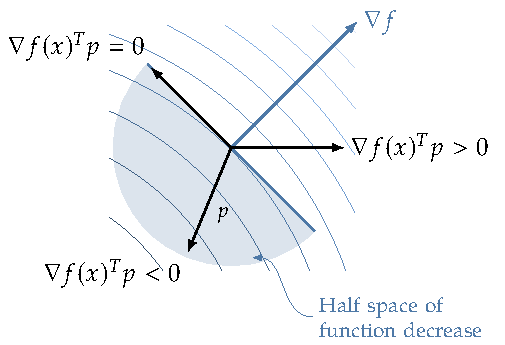
\includegraphics[width=3.0in]{gradf_half_space}
	\caption{This is a regular figure with a centered bottom caption.}
	\label{fig:gradf_half_space}
\end{figure}

\myshorttext

With the {\ttfamily byuthesis.cls} document class, we can have small figures that are set in the sidemargin. Figure~\ref{fig:brach} is an example of a margin figure.
\begin{marginfigure}
	\includegraphics[width=1.8in]{brachistochrone}
	\caption{This is an example of a margin figure.}
	\label{fig:brach}
\end{marginfigure}

\myshorttext

We can also create figures that place the caption in the side margin. This is a matter of personal preference.
\begin{figure}[htbp]
	\begin{sidecaption}{This is a figure with a side caption that is not short, but not that long either.}[fig:sidecap]
		\centering
		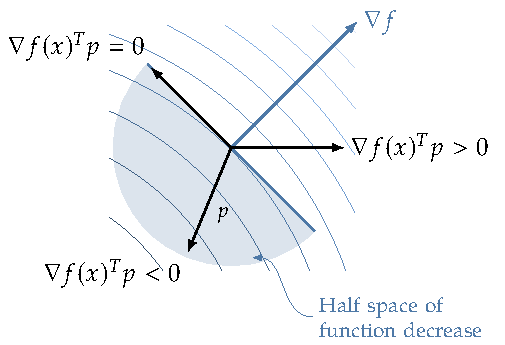
\includegraphics[width=3.5in]{gradf_half_space}
	\end{sidecaption}
\end{figure}

Finally, we can create a figure that spans the width of the text column and the side margin. This option should not be used frequently as it requires some tweaking of the vertical distance of the caption and follow-on text below the figure. It will work robustly when the figure appears at the top or middle of a page, but may push the caption onto the next page when it appears at the bottom. There may be some instances with wide images where the additional manual adjusting is worth the effort.

\begin{figure}[h]
	\setlength{\sidecapraise}{-1.3cm}   % manual adjustment of figure caption position
	\begin{sidecaption}{The caption for a full-width figure appears in the margin below it.}[fig:fullwidth] %Such figures utilize the side margin.}
		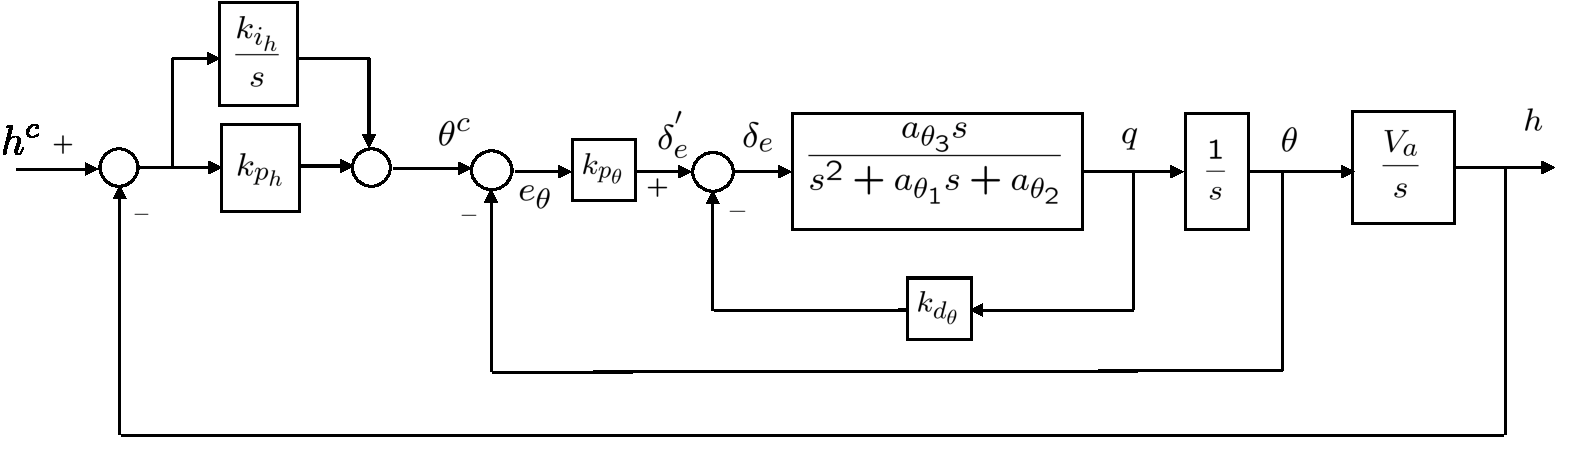
\includegraphics[width=1.35\textwidth]{altitude-pitch-all}
	\end{sidecaption}
	\vskip -1.7cm     % manual adjustment of position of main text below figure   
\end{figure}

\subsubsection{Subsubsection Example}
The syntax above provides an example of how to include a subsubsection. In this thesis template, the document has four primary division levels: \verb|\chapter|, \verb|\section|, \verb|\subsection|, and \verb|\subsubsection|. The command \verb|\subsubsection| is used to define the lowest level of division. Notice that subsubsection titles are not numbered.

\subsubsection{Including Tables}
Tables are also fairly straightforward to include in a \LaTeX{} document. Table~\ref{tab:table_example} shows a simple table. \LaTeX{} refers to figures and tables as floats and often tries to locate figures at the top or bottom of a page. The user has some control over this, but \LaTeX{} can behave like it has a mind of its own sometimes. In reality it is placing figures according to internal algorithms and parameters that you can adjust. If you are interested in digging into this level of detail, an internet search on ``LaTeX float parameters'' will provide ample reading.  In creating the table, we have used the command \verb|\begin{table}[t]|. The parameter \verb|[t]| allow us to specify preference for the location of table to be at the \emph{top} of the page.

\begin{table}[t]
	\centering
	\caption{This is a standard table with a top caption.}
	\label{tab:table_example}	\begin{tabular}{ c c c c}
		\toprule
		basin & curve \\
		name & number & minimum & maximum \\
		\midrule
		1B & 68.5 & 49.2 & 84.1 \\ 
		2B & 66.2 & 46.8 & 82.7 \\ 
		3B & 65.4 & 45.5 & 82.3 \\
		\midrule
		average & 66.7 & 47.2 & 83.0 \\
		\bottomrule
	\end{tabular}
\end{table}

Table~\ref{tab:table_sidecaption} shows an example of the same table using a side caption. We have used the placement preferences \verb|[thb]| to give first preference to the top of the page, second preference to the current positioning in the source code (\emph{here}), and third preference to the \emph{bottom} of the page. As you can see, \LaTeX{} may override our preferences, based on the space available and its typesetting rules.
\begin{table}[thb]
	\begin{sidecaption}{This is a standard table with a side caption.}[tab:table_sidecaption]
		\centering
		\begin{tabular}{ c c c c}
			\toprule
			basin & curve \\
			name & number & minimum & maximum \\
			\midrule
			1B & 68.5 & 49.2 & 84.1 \\ 
			2B & 66.2 & 46.8 & 82.7 \\ 
			3B & 65.4 & 45.5 & 82.3 \\
			\midrule
			average & 66.7 & 47.2 & 83.0 \\
			\bottomrule
		\end{tabular}
	\end{sidecaption}
\end{table}

\subsection{Formatting Equations}
Equation formatting is one of \LaTeX's most useful features and a good reason why it is often used for theses and dissertations in the College of Engineering. It is easy to format equations within a sentence, such $c = 2 \pi r$ to describe the circumference of a circle. Equations should be treated as part of the text. As an example, the surface area of a cylinder is given by 
\begin{equation}
	\label{eq:surface_area_cyl}
	S = 2\pi r \left( r + h \right) , 
\end{equation}
where $r$ is the radius of the cylinder and $h$ is its height. The area of a circle can be expressed in terms of its diameter $d$ as 
\begin{equation}
	\label{eq:area_circle}
	A = \frac{\pi}{4} d^2 .
\end{equation}

Often, it is desirable to align a sequence of equations. Again, \LaTeX{} makes this pretty easy. The roots of the polynomial function $f(x)$ can be found by factoring
\begin{align}
	f(x) &= x^3 + 5x^2 + 6x \\
		 & = x (x^2 + 5x + 6) \\
		 & = x (x + 2)(x +3) ,
\end{align}
setting each of the factors to zero, and solving for $x$. Equations without numbers can be typeset like this
\[
	x = a + b
\]
or like this
\begin{equation*}
	y = c + d .
\end{equation*}
Just as we did with sections, figures, and tables, we can reference a specific equation by using its declared label. In~\eqref{eq:surface_area_cyl}, the surface area of a cylinder is defined. Another format would be to say Equation~\ref{eq:area_circle} defines the area of a circle. Yet another format is \cref{eq:area_circle}. Any of these formats is acceptable. Use just one of them and be consistent.

\LaTeX{} can do so much with the typesetting of equations. These few examples are just a small sampling of its impressive capabilities.


%	\chapter{Additional \rmfamily{\LaTeX{}} Formatting}
\label{ch:ch2}

In this chapter, we'll provide some additional guidelines and useful \LaTeX{} commands for formatting your document.


%{\color{mediumgray} \blindtext}
\section{More {\rmfamily\LaTeX{}} Usage Examples}
In Figure~\ref{fig:brach2} below, we show some pretty blue and grey lines. This is the first figure in \cref{ch:ch2} and you can see that it is numbered accordingly. Notice that the \verb|\ref| command automatically provides the correct numbering for the item being referenced. If you use the \verb|\cref| command, the label (e.g., Figure, Chapter) will be added automatically. For figures and equations, however, \verb|\cref| will abbreviate the labels (i.e., Fig. and Eq.). Either \verb|\ref|, with label provided by you, or \verb|\cref|, with automatic labeling, can be used. 

\begin{figure}[htbp]
	\centering
	\includegraphics[width=2.2in]{figures/brachistochrone}
	\caption[Short caption to appear in list of figures.]{This is another figure. Some authors have paragraph-like descriptions of their figures that they put into the caption. This is acceptable, but readers don't really want or need a super long caption showing up in their list of figures. The {\ttfamily caption} command provides a nice solution.}
	\label{fig:brach2}
\end{figure}

\section{Bibliography}
Another great feature of \LaTeX{} is that it allows you to create a list or database of books, papers, and other documents that you can easily cite in your document. In engineering, it is common to give your bibliography list the title References and we will follow that convention. \LaTeX{} automatically numbers the citations and builds a bibliography for you.\sidenote{The building of your bibliography is actually done by the {\ttfamily biblatex} package. If you use an IDE to work with \LaTeX, this may not be obvious to you.} The bibliography is typeset according the style you specify. We recommend the {\em IEEEtran} bibliography style that produces a numbered list in order of citation. For this document, the file {\ttfamily references.bib} contains the bibliographic reference information that's available for citation in the thesis document. Each reference is given a cite key (a label) that is used to cite the reference. For example, here is a reference to a book~\autocite{book1} and a reference to a doctoral dissertation~\autocite{doctoral1}. Journal articles~\autocite{journal1}, are treated differently than conference papers~\autocite{conference1} since their references require slightly different information. For each reference entry in your {\ttfamily .bib} file, different information fields will have to be populated. Examples of these fields include, {\em author}, {\em title}, {\em year}, and so on. Different types of publications will have different required fields for you to fill out. There are other types of citations that you may use, such as book chapters and websites. You can manually edit your {\ttfamily .bib} file with a text editor, or you can use one of the several popular apps that are available for editing and organizing your bibliography information.

\section{Use of Units}
Units should be appropriately used for all measurements and data presented in the document. Standard abbreviations for units (e.g., m for meters, N for newtons, in. for inches) should be used whenever data is presented. For example, the shaft was 1.23 cm in diameter. Notice that there is a space between the number and the unit, and the unit is typeset in vertical (roman) text and is {\em not italicized}. Italics is reserved for emphasis and for mathematical variables. Periods are not used after abbreviations except in the special case of the abbreviation for inches as in. to avoid confusion with the word in. Units are typically spelled out when they are used without data. For example, newtons are a measure of force, while kilograms are a measure of mass.

\section{Capitalization of Reference Labels}
Throughout your document, you will refer to figures, tables, equations, chapters, appendices, and sections by name (e.g., Figure 2.1, Section 3.4, Equation 2.1, and so on). You may choose to capitalize these reference labels, or to leave them uncapitalized (e.g., figure 2.1, section 3.4, equation 2.1). The choice is yours, just be consistent -- all reference labels should be capitalized, or uncapitalized.

\section{Algorithms}
Software and algorithm development can play an important role in graduate research. Rather than including software code, particularly in the body of the thesis, presenting your algorithms in the form of pseudo-code may be more desirable. The {\ttfamily algorithm} package in \LaTeX{} provides tools for clearly presenting your algorithms. A simple example of the use of this package is presented in Algorithm~\ref{alg:ekf}.

\begin{algorithm}
	\caption{{\color{black} Continuous-discrete extended Kalman filter.}} \label{alg:ekf}
	\begin{algorithmic}[1]
	    \State Initialize:  $\hat{x} = 0$.
	    \State Pick an output sample rate $T_{\textit{out}}$ that is much less than
	    the sample rates of the sensors.
	    \State At each sample time $T_{\textit{out}}$:
	    \For{$i=1$ to $N$}
	        \State $\hat{x} = \hat{x} + \left(\frac{T_{\textit{out}}}{N}\right) \left( f(\hat{x}, u)\right)$
	        \State $A = \frac{\partial{f}}{\partial{x}}$
	        \State $P = P + \left(\frac{T_{\textit{out}}}{N}\right)
	        \left(AP+PA^T + GQG^T\right)$
	    \EndFor
	    \If{a measurement has been received from sensor $i$}
	        \State $C_i = \frac{\partial{c_i}}{\partial{x}}$
	        \State $L_i = PC_i^T(R_i+C_iPC_i^T)^{-1}$
	        \State $P = (I-L_iC_i)P$
	        \State $\hat{x} = \hat{x} +  L_i\left( y_i - c_i( \hat{x})
	        \right)$.
	    \EndIf
	\end{algorithmic}
\end{algorithm}

\section{Landscape Drawings and Tables}
If you have a figure or table that is best presented in landscape format on a full page, the {\ttfamily rotating} package in \LaTeX{} provides a convenient way to do this. Figure~\ref{fig:landscape_dwg} on the following page shows an example a landscape-format drawing.
\begin{sidewaysfigure}
	\centering
	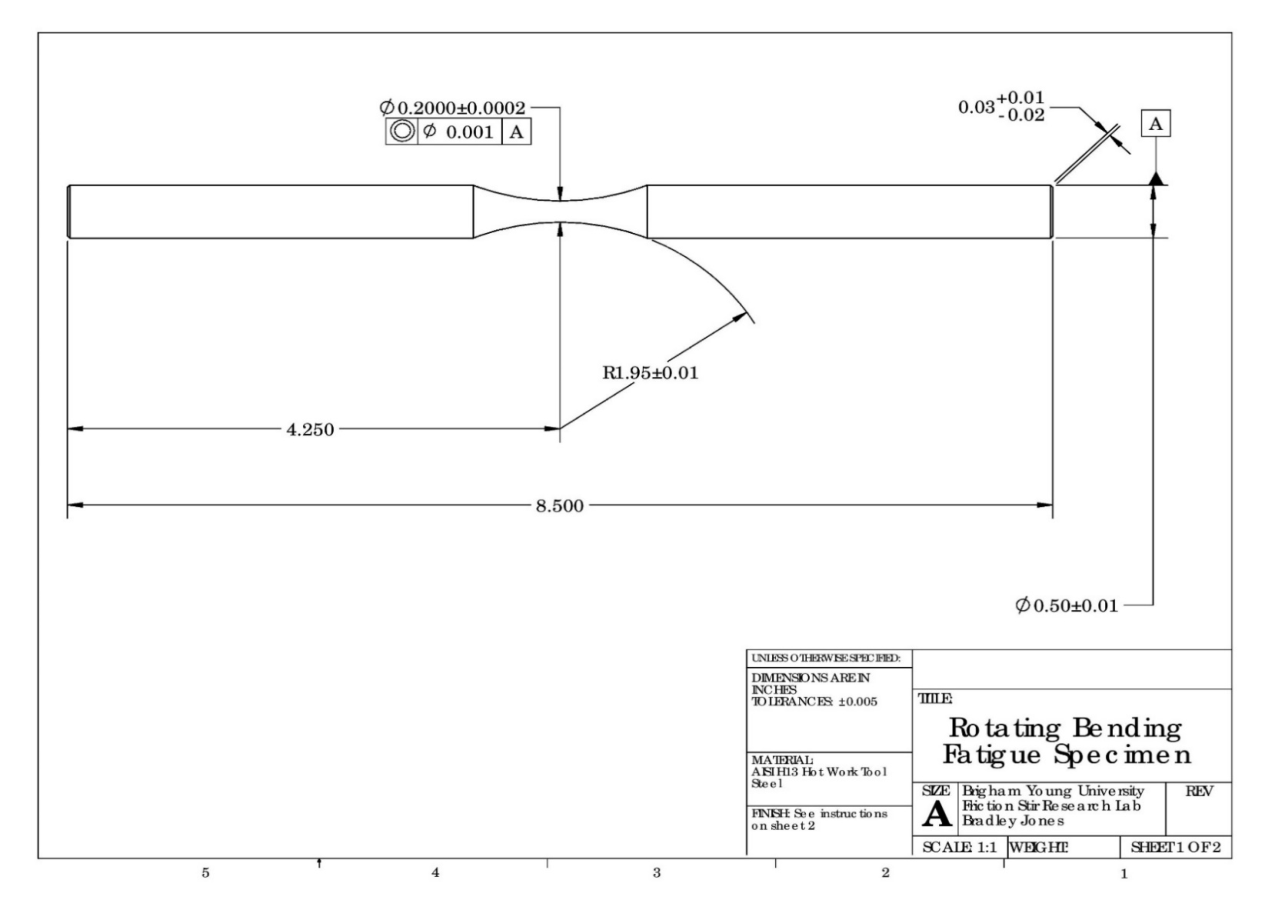
\includegraphics[width=0.7\textwidth]{figures/part_dwg_landscape.pdf}
	\caption{Example of full-page landscape drawing.}
	\label{fig:landscape_dwg}	
\end{sidewaysfigure}



%	\chapter{Article-based Chapters}
\label{ch:article_based_chap}

With the allowed changes in thesis and dissertation formatting, BYU Graduate Studies
now allows students to insert journal or conference articles as chapters into their
thesis/dissertation document. To do so, the student must be a primary author. The
formatting of an article-based chapter must be fully consistent with the formatting
defined in this document with chapter, section, equation, figure, and table numbering
integrated accordingly. Article-based chapters must include a complete citation and
the following statement: ``I hereby confirm that the use of this article is compliant
with all publishing agreements.'' The paragraph below is an example of how this could
be done. It should appear immediately following the chapter title.

\noindent This chapter is composed from a paper entitled ``Really great research from
a BYU engineering student'' published in the journal Awesome Engineering~\cite{StudentRP20}.
I hereby confirm that the use of this article is compliant with all publishing agreements.

\section{Some Additional Comments}
The publication of a conference or journal article is a significant milestone for a graduate 
student and should be an objective for all students pursuing graduate research in the College 
of Engineering. We encourage the use of article-based chapters in theses and dissertations 
provided that it aligns with the goals and objectives of the research. Articles, however, 
are often constrained in length forcing the exposition to be more concise or narrow in 
scope than may be desired for the intended audience of the thesis/dissertation. For example, 
if an objective is to guide the learning of subsequent graduate-student researchers, it 
may be beneficial to include additional details or a broader discussion that may be more 
tutorial in nature. Often more results from a wider variety of cases would be included 
in a dissertation or thesis than would be possible in a journal or conference publication. 
Your graduate committee will help guide your efforts in these matters.

%	\chapter{Conclusions}

The purpose of this template is to provide basic instructions in creating your dissertation/thesis document. If you need assistance with writing, please visit the Writing Center in the JKB or consult with your advisor. If you need assistance with \LaTeX, there are tutorials and ample documentation online. You may want to consult with your graduate-student peers who use \LaTeX. If you discover something that would make this template more useful, please feel free to make recommendations.

Regardless of whether this template or some other method of formatting is employed, you (the student) are responsible for following the guidelines found in \cref{ap:format}. Below is a brief checklist of things to look for as you review your thesis for formatting:
\begin{itemize}
	\item Check numbering of sections, figures, tables, equations to make sure they are consistent.	This is where you will be really glad that you are using \LaTeX.
	\item Ensure that your table of contents, list of figures, and list of tables are up to date and that page numbers are correct. (Hurray for \LaTeX!)
	\item Make sure all pages are numbered, beginning with the table of contents.
	\item Be sure there is no more than 1 inch of extra white space at the bottom of any page (in addition to the 1-inch margin) except for the final page of a chapter.
	\item Make sure there are no widows or orphans.\footnote{A \emph{widow} occurs when the last line of a paragraph ends up on the first line of a page. An \emph{orphan} occurs when the first line of a paragraph appears on the last line of a page. Your document may require manual tweaking when it is in final form to get rid of widows and orphans.}
\end{itemize}




%%%%%%%%%%%%%%%%%%%%%%%%
% --- Bibliography --- %
%%%%%%%%%%%%%%%%%%%%%%%%
	\printbibliography[title=References]


%%%%%%%%%%%%%%%%%%%%%%
% --- Appendices --- %
%%%%%%%%%%%%%%%%%%%%%%
	\appendix

	\chapter{Electronic Document Submission}
\label{ap:elect_doc}

The university requires all dissertations and theses to be submitted electronically as 
a PDF document. All required fonts should be embedded in the PDF document to ensure that
your document will appear as intended wherever it is viewed. You can verify that all fonts
are appropriately embedded by opening your PDF document in Adobe Acrobat Reader and selecting
{\ttfamily{File->Properties}}. Under the Font tab, you should see a list of the fonts used in your document.
To ensure that all fonts are embedded, they should be designated as ``Embedded" or ``Embedded 
Subset" in the list.

\section{PDF Bookmarks}
The PDF document must contain bookmarks for preliminary pages plus chapter headings and 
subheadings, as listed in the Table of Contents. In the PDF document, bookmarks should be 
displayed in a panel to the left of the document pages as seen in Figure~\ref{fig:PDF_doc}. 

\begin{figure}[htbp]
\centering
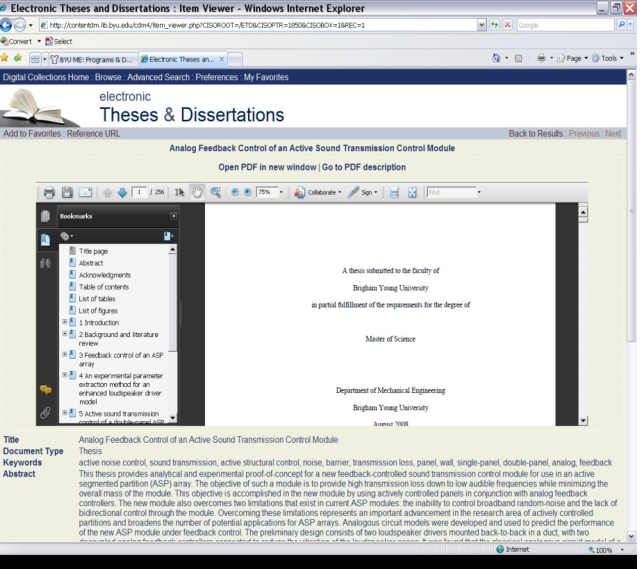
\includegraphics[width=4.5in]{figures/PDF_doc}
\caption{PDF thesis document showing ETD bookmarks.}
\label{fig:PDF_doc}
\end{figure}

If assistance is needed with embedding, bookmarks, or other aspects of submitting the ETD, 
you may obtain assistance at the Multi-media lab in the HBLL. Please note that keywords for 
your research, as listed at the bottom of Figure~\ref{fig:PDF_doc}, will be required at the
time you submit your document. Keywords must be in lower case, unless they are acronyms or 
proper nouns. In addition, a copy of the abstract must be inserted.

Tables and figures appearing in appendices should be numbered A.1, B.1, etc. and should be 
included in the lists of tables and figures.

\section{Miscellaneous Filler}
Most appendices will be longer than 3/4 of a page. We'll use some Latin to fill this one out. {\color{mediumgray} \blindtext}




	\chapter{Electronic Document Submission}
\label{ap:elect_doc}

The university requires all dissertations\scite{bugref1,bugref2} and theses to be submitted electronically as a PDF document. All required fonts should be embedded in the PDF document to ensure that your document will appear as intended wherever it is viewed. You can verify that all fonts are appropriately embedded by opening your PDF document in Adobe Acrobat Reader and selecting {\ttfamily{File->Properties}}. Under the Font tab, you should see a list of the fonts used in your document. To ensure that all fonts are embedded, they should be designated as ``Embedded'' or ``Embedded Subset'' in the list.

\section{PDF Bookmarks}
The PDF document must contain bookmarks for preliminary pages plus chapter headings and subheadings, as listed in the Table of Contents. In the PDF document, bookmarks should be displayed in a panel to the left of the document pages as seen in Figure~\ref{fig:PDF_doc}. 

\begin{figure}[htbp]
	\centering
	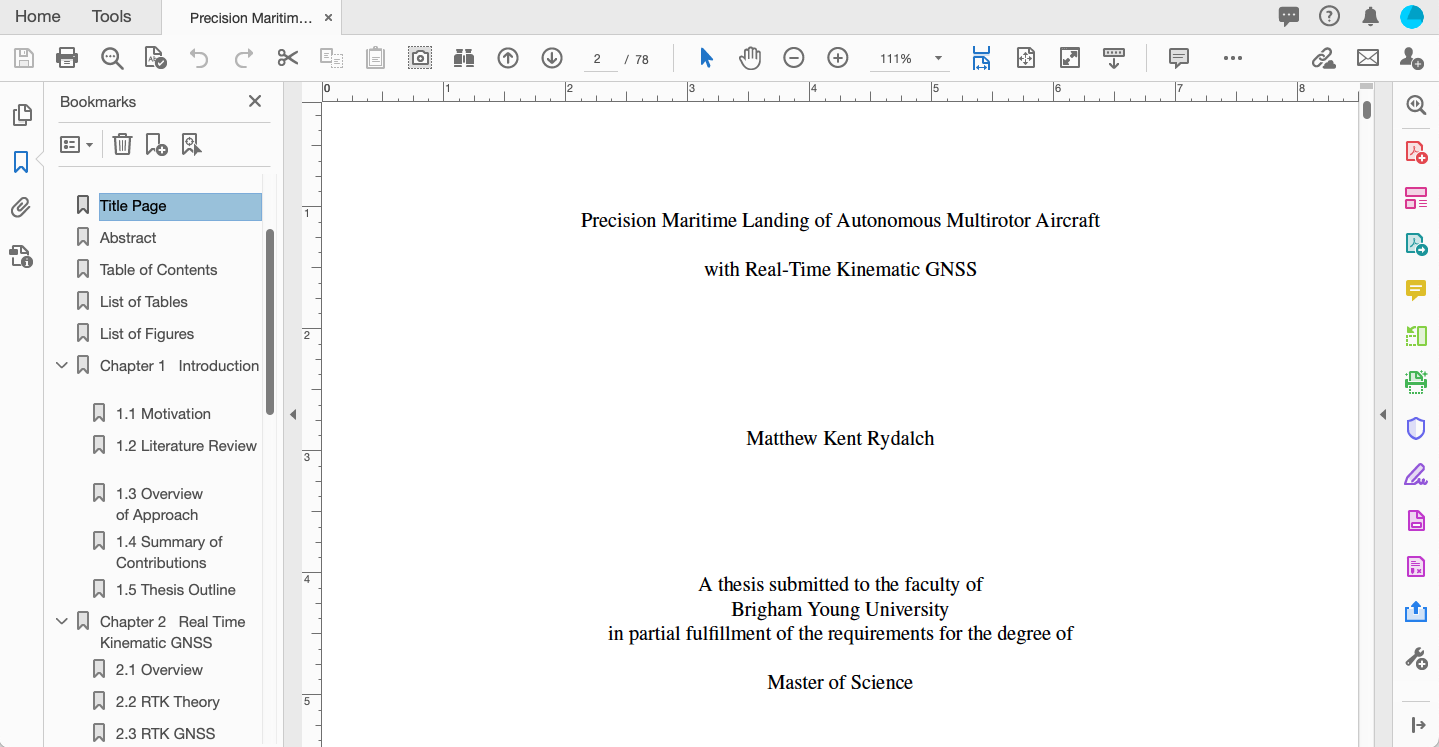
\includegraphics[width=4.5in]{figures/ETD_thesis}
	\caption{PDF thesis document showing ETD bookmarks.}
	\label{fig:PDF_doc}
\end{figure}

If assistance is needed with embedding, bookmarks, or other aspects of submitting the ETD, you may obtain assistance at the Multimedia Lab in the HBLL. Please note that keywords for your research will be required at the time you submit your document. Keywords must be in lower case, unless they are acronyms or proper nouns. In addition, a copy of the abstract must be inserted. Helpful information on submitting your ETD copy can be found at \url{https://gradprogress.sim.byu.edu/resources}.

\section{Miscellaneous Filler}
Most appendices will be longer than 3/4 of a page. We'll use some Latin to fill this one out. {\color{mediumgray} \blindtext}




	\chapter{Document Formatting}
\label{ap:formatting}

\section{Font Selection}
	Font must be a conservative serif-styled font (e.g., Palatino, Times New Roman, Garamond), size 11 pt. The font style and size must be consistent throughout the text. 10 pt. font is allowed for figure and text captions. The font size for figures should be no smaller than 8 pt. and easily legible.

	\section{Document Margins}
	Front matter pages (title page, abstract page, acknowledgment page)
	\begin{itemize}
		\item 1-inch top and bottom margins
		\item 2-inch left and right margins
	\end{itemize}

	\noindent Table of contents, list of figures, list of tables, body pages
	\begin{itemize}
		\item 1-inch top and bottom margins
		\item 2-inch left and right margins
	\end{itemize}

	\noindent Chapter title pages, reference title page, appendix title pages
	\begin{itemize}
		\item 2-inch top margin
		\item 1-inch bottom margin
		\item 2-inch left and right margins
	\end{itemize}

	\section{Printing Instructions}
	Not all departments require a printed and bound copy of the thesis document. If a bound copy of the document is required, it should be printed double-sided. Please note that following pages must begin on recto page: title, abstract, acknowledgment, table of contents, list of figures, list of tables, chapter title, references, and appendix title.

	\section{Page Numbering}
	\begin{itemize}
		\item Page numbers are centered at the bottom of the page.
		\item Counting begins with the title page
		\item Page numbers do not appear until after the table of contents.
		\item Use Roman numerals (e.g., i, ii, iii, etc.) for the table of contents and the pages thereafter until Chapter 1 begins.
		\item Use Arabic numbers (e.g., 1, 2, 3 etc.) beginning with Chapter 1. Be sure numbers appear on {\em all} non-blank pages once numbering begins.
	\end{itemize}

	\section{Line Spacing}
	The document should be single spaced with the exception of space around titles, headings, subheadings, figures, tables, and equations as described below. Please note that the document style of this template  has been defined to conform to these requirements.
	\begin{itemize}
		\item Two-inch margin above chapter titles (144 pts).
		\item One inch of space after chapter titles (72 pts).
		\item 18 pts before level 2 subheadings.
		\item 6 pts after level 2 subheadings.
		\item 12 pts before level 3 subheadings.
		\item 3 pts after level 3 subheadings.
		\item 12 pts (1 carriage return with 11-pt font) before figures
		\item 9 pts between figure and caption, 15 pts between figure and following text.
		\item 9 pts before table caption, 3 pts between caption and table.
		\item 12 pts between table and following text.
		\item 6 pts before and after equations.
		\item Do not leave a single line of text or a subheading alone on the top (widow) or bottom (orphan) of a page.
		\item Do not leave more than 1 inch of extra white space remaining on the bottom of a page unless it is at the end of a chapter. An exception to this rule is for pages containing no text and only figures and tables.
	\end{itemize}
	
	\section{Figure Formatting}
	\begin{itemize}
		\item Figures are typically diagrams, graphs, pictures, maps, or charts.
		\item Center figures on the page.
		\item Center captions below the figure. If multiple lines are needed, the caption should be left/right justified at the margins.
		\item A figure should be placed after the paragraph in which it is first referenced. If it will not fit on the same page, continue the text and place the figure at the top of the next page.
	\end{itemize}
	
	\section{Table Formatting}
	\begin{itemize}
		\item Tables typically contain numerical or statistical information.
		\item Center tables on the page.
		\item Center captions above the table, not to exceed the width of the table. If multiple lines are needed, the caption should be left/right justified at the margins, such as
	\end{itemize}
	
	\noindent Table 6.3: Comparison of roll rotation plots when spatial node was displaced, and an X-direction force was applied.
	
	\begin{itemize}
		\item If placed in the landscape position, the top of the table should be on the left side of the page, with the caption above the table. The page number is placed underneath the table.
	\end{itemize}



%%%%%%%%%%%%%%%
% --- End --- %
%%%%%%%%%%%%%%%
\end{document}

